% !TeX program = lualatex
% !TeX encoding = UTF-8
% !TeX spellcheck = fr_FR

% Packages classiques
\documentclass[french]{article}
\usepackage[utf8]{inputenc}
\usepackage[T1]{fontenc}
\usepackage[left=2cm, right=2cm, top=2cm, bottom=2cm]{geometry}
\usepackage{polyglossia}
\usepackage{mathtools, amssymb, amsmath, amsthm}
\usepackage{caption}
\usepackage{footnote}
\usepackage{hyperref}
\usepackage{multicol}
\usepackage{array}
\usepackage[backend=biber,style=alphabetic, maxnames=6, maxalphanames=6, maxcitenames=6]{biblatex}

% Packages graphiques
\usepackage{xcolor}
\usepackage{graphicx}
\usepackage{tikz}
\usepackage{pgfplots}
\usepackage{subfigure}
\pgfplotsset{width=10cm,compat=1.9}

% Paramètres
\usepackage{microtype}
\definecolor{vert}{RGB}{0, 153, 0}
\definecolor{gris}{RGB}{50,60,200}
\hypersetup{
    colorlinks=true,
    citecolor=vert,
    linkcolor=gris,
    urlcolor=gris
}
% Adjust formatting for specific keywords
\addbibresource{biblio.bib}

% Labelling automatique
\let\orisectionmark\sectionmark
\renewcommand\sectionmark[1]{\orisectionmark{#1}\label{sec:#1}}
\let\orisubsectionmark\subsectionmark
\renewcommand\subsectionmark[1]{\orisubsectionmark{#1}\label{subsec:\thesection.#1}}
\let\orisubsubsectionmark\subsubsectionmark
\renewcommand\subsubsectionmark[1]{\orisubsubsectionmark{#1}\label{subsubsec:\thesection.\thesubsection.#1}}
\let\oldtheequation\theequation
\makeatletter
\def\tagform@#1{\maketag@@@{\ignorespaces#1\unskip\@@italiccorr}}
\renewcommand{\theequation}{(\oldtheequation)}
\makeatother 
\renewcommand{\tableautorefname}{Tab.}
\renewcommand{\theoremautorefname}{Théorème}

% Commandes pour les thm
\newtheorem{thm}{Théorème}[section]
\newcommand{\thmautorefname}{Théorème}
\newtheorem{cor}{Corollaire}[thm]
\newcommand{\corautorefname}{Corollaire}
\newtheorem{lemma}[thm]{Lemme}
\newcommand{\lemmaautorefname}{Lemme}
\newtheorem{prop}{Propriété}[section]
\newcommand{\propautorefname}{Propriété}
\newtheorem{Def}{Définition}[section]
\newcommand{\Defautorefname}{Définition}
\newtheorem{example}{Exemple}[section]
\newcommand{\exampleautorefname}{Exemple}

\renewcommand{\subsectionautorefname}{Section}
\renewcommand{\subsubsectionautorefname}{Section}

%input files
\makeatletter
\makeatother
\graphicspath{{../figures/}}

\title{Projet CGDI : Générateurs de longueur minimale sur les surfaces}
\author{Adrien Dubois}
\date{\today}

\begin{document}

\maketitle
\begingroup 
\hypersetup{linkcolor=black}
\tableofcontents
\endgroup

\section{Motivation}

\subsection{Contexte}

\indent L'étude et la classification des variétés en topologie sont des sujets très explorés en mathématiques, bien que leur complexité soit indéniable. 
Contrairement aux défis rencontrés dans des espaces de dimension supérieure, 
comme en témoigne la conjecture de Poincaré, 
la topologie des variétés en dimension 2 est bien maîtrisée et documentée, 
facilitant ainsi la résolution de problèmes algorithmiques dans ces contextes. 
De plus, les surfaces de dimension 2 dans l'espace à 3 dimensions représentent des entités réelles avec des applications potentielles dans des domaines tels que l'optimisation, l'ingénierie, et l'imagerie numérique. 
Nous nous concentrerons donc sur une problématique liée à ces objets.

\subsection{Sujet}

L'idée serait de trouver les générateurs les plus courts d'une surface dans $\mathbb{R}^3$. 
Par plus court, on entend minimiser la somme des longueurs des cycles.
Plus précisemment, le sujet est le suivant:

\begin{center}
    Soit $S$ une 2-variété connexe, compacte, orientable et sans bord. \newline
    Trouver une base de cycles générateurs de $S$ dont la somme des longueurs est minimale.
\end{center}
autrement dit un ensemble de cycles dont les classes d’homologie génèrent le $1^{er}$ groupe d’homologie de $S$.

\subsection{État de l'art}

Un problème plus général est de trouver la coupure de graphe de longueur minimale pour obtenir un disque topologique.
Erickson et Har-Peled ont montré que ce problème est NP-dur. Il est à noter que la difficulté vient du fait que le graphe considéré est général. \\
Colin de Verdière et Lazarus \cite{loops} se sont ensuite intéréssés aux coupures de graphes en les sommets, appelés systèmes de boucles, de longueur minimales sur les surfaces orientables et sans bords.
C'est un cas particulier de ce sujet, à voir en détail dans la \autoref{sec:Définitions}. \\
Le problème concerné dans ce sujet a été étudié par Erickson et Whittlesey \cite{erickson_whittlesey}, pour les classes homotopiques et homologiques. 
Leur algorithme permet de trouver une base d'homotopie (voir \autoref{subsec:2.Boucles, Systèmes de boucles et Homotopies}) en temps $O(n \log n)$ ainsi que les générateurs d'une surface en $O(n^2 \log n + n^2g + ng^3)$ si $n$ est le nombre de sommets et $g$ le genre de la surface. \\
Pour finir, une implémentation a été réalisée par \cite{implementation}, qui reprend dans les grandes lignes l'algorithme de Erickson et Whittlesey, sans pour autant fournir les détails de l'implémentation ou le code source.
L'implémentation réalisée jointement à ce rapport ne provient pas d'une source extérieure, et est simplement basée sur les preuves de l'article \cite{erickson_whittlesey}.

\section{Définitions}

On commence par définir les notions de topologies qui seront utiles à exploiter dans les algorithmes dans la suite

\subsection{Généralités topologiques}

\begin{Def}[2-variété]
Une variété 2-dimensionnelle est un espace dans lequel chaque point a un voisinage homéomorphe au plan euclidien $\mathbb{R}^2$.
\end{Def}

\begin{Def}[Genre]
Le genre d'une surface est le nombre maximal de cycles disjoints qui peuvent être enlevés sans déconnecter la surface.
\end{Def}

\begin{prop}[Classification des 2-variétés \cite{class_surfaces}]
    Toute 2-variété compacte et sans bords est homéomorphe à l'un des objets suivants:
    \begin{itemize}
        \item une 2-sphère
        \item une somme connexe de $g$ tores, dit $g$-tore (cas orientable avec surface de genre $g$)
        \item une somme connexe de plans projectifs (cas non-orientable)
    \end{itemize}
\end{prop}

Ce sujet concerne les surfaces qui appartiennes à la première ou deuxième catégorie
dites 2-variétés compactes, orientables et sans bords.
On peut alors les classifier selon leur genre $g$. \\
Dans le reste du rapport, on appelera "surface" une variété 2-dimensionnelle compacte, orientable, sans bords. 
Par souci de simplicité, les définitions et propriétés concernent en général les surfaces continues, 
mais cela s'étend aux cas discrets des maillages.

\begin{prop}
    Une surface vérifiant les conditions ci-dessus de genre $g$ possède $2g$ générateurs.
\end{prop}

\begin{Def}[Caractéristique d'Euler]
    On définit la caractéritique d'Euler sur les maillages comme $\chi = V-E+F$ avec $V$ le nombre de sommets, $E$ le nombre d'arêtes et $F$ le nombre de faces.
\end{Def}

\begin{prop}
    Pour les surfaces vérifiant les conditions précédentes et de genre $g$, $2-\chi = 2g$ 
\end{prop}

\subsection{Boucles, Systèmes de boucles et Homotopies}

\begin{Def}[Boucle d'origine $x$]
Soit $S$ une surface. Une boucle d'origine $x \in S$ est l'image d'une fonction continue de $[0,1]$ dans $S$ 
dont le point de départ et le point d'arrivée sont identiques ($x$). 
Elle est dite rétractable si elle peut être déformée de manière continue en un point.
\end{Def}

\begin{Def}[Relation d'équivalence, homotopie]
    Deux boucles sont équivalentes ou homotopes si l'une peut être continuement déformée sur l'autre.
\end{Def}

\begin{Def}[Système de boucles]
    Un système de boucles est un ensemble de boucles simples dont la suppression dans la variété laisse un espace homéomorphe à un disque.
\end{Def}

\begin{Def}[Groupe fondamental]
Le groupe fondamental d'une variété (surface) est un l'ensemble des classes d'équivalences (dites classes homotopes) 
des boucles. 
Il est souvent noté $\pi_1(S,x)$ où $S$ est la variété et $x$ la source, point d'intersection des boucles.
\end{Def}

\begin{Def}[Base d'homotopie \cite{erickson_whittlesey}]
Une base d'homotopie est un ensemble de boucles dans une variété qui génère son groupe fondamental.
\end{Def}

Dans la \autoref{subsec:3.Base d'homotopie gloutonne}, on donne un algorithme pour calculer une telle base en $O(n \log n)$ où $n$ est le nombre de sommets.

\subsection{Cycles et Homologies}

\begin{Def}[Cycle]
    On appelle cycle une boucle considérée indépendamment dans sa source.
\end{Def}

Dans la suite, il est question des groupes d'homologies d'un espace topologique $X$. Informellement, le $k^e$ groupe d'homologie de $X$, $H_k(X)$, décrit les "trous" de dimension $k$ dans $X$. 
Par exemple, le premier groupe d'homologie $H_1(X)$ décrit les classes d'équivalences des cycles de $X$ donc les "trous" d'une surface.

\begin{Def}[Base d'homologie \cite{erickson_whittlesey}]
Une base d'homologie est un ensemble de cycles dans une variété $S$ qui génère son premier groupe d'homologie $H_1(S)$,
aussi appelés plus simplement les générateurs de la surface.
\end{Def}

\subsection{Propriétés utiles}

\begin{prop}
    Un système de boucles est aussi une base d'homotopie. Une base d'homotopie est aussi une base d'homologie.
\end{prop}

\begin{Def}["Reduced cut locus"]
Le "reduced cut locus" de base $x$ d'une variété est l'ensemble des points 
qui peuvent être atteints à partir de $x$ par au moins deux chemins les plus courts 
qui ne sont pas homotopiquement équivalents.
\end{Def}

\noindent \textbf{Remarque :} Pour nos maillages, ces points ne sont en général pas des sommets mais des points le long d'arêtes. 
C'est pourquoi on considérera le "reduced cut locus" plutôt comme un ensembles d'arêtes contenant les points en question.

\begin{prop}
    Tout cycle coupe au moins le "reduced cut locus" une fois
\end{prop}

\noindent On note $\sigma(c,x)$ la fonction qui associe à un point $x$ et à un élément du "reduced cut locus" $c$ 
la boucle la plus courte et non rétractable qui contient ces deux éléments.

\begin{prop}
    Soit $S$ une surface, $x \in S$ et $\Phi(S, x)$ son "reduce cut locus". Alors tout boucle de $S$ dans la plus courte base d'homotopie s'écrit $\sigma(x, e)$ avec $x \in S$ et $e \in \Phi(S, x)$
\end{prop}

\section{Algorithme, Complexité et Implémentation}

\subsection{Base d'homotopie gloutonne}

\begin{Def}[Base d'homotopie gloutonne \cite{erickson_whittlesey}]
    \label{Def: base_homotopie_g}
    Soit $S$ une surface de genre $g$ et $x \in S$ une source. 
    La base d'homologie gloutonne est l'ensemble $\{\gamma_1(x), ..., \gamma_{2g}(x)\}$ tel que :
    \begin{align*}
        \forall i \in \{1, ..., 2g\},\ \gamma_i 
        \text{ est la boucle } l(x) \text{ d'origine } x \text{ la plus courte telle que }
        M \setminus (\gamma_1(x) \cup ... \gamma_{i-1}(x) \cup l(x))
        \text{ est connexe}
    \end{align*}
\end{Def}

\begin{thm}[\cite{erickson_whittlesey}]
    L'ensemble des sous-ensembles de bases homotopiques n'est pas un matroïde
\end{thm}

A priori, la base homotopique n'est donc pas de longueur minimale ou on ne peut du moins pas l'avoir directement avec les matroïdes. 
Cependant, Erickson et Whittlesey donnent la preuve de son optimalité.

\begin{thm}[\cite{erickson_whittlesey}]
    Soit $S$ une surface de genre $g$ et $x \in S$ une source.
    La longueur de la base d'homologie gloutonne est minimale pour les bases d'homologie générant le groupe fondamental $\pi_1(S, x)$
\end{thm}

\subsection{Calcul de la base d'homotopie gloutonne}

Intéressons nous maintenant aux détails de l'implémentation. 
Appliquer directement la \autoref{Def: base_homologie_g} pour trouver la base serait trop couteux.
En effet, il faudrait calculer $l$ comme cycle non rétractable le plus court à l'aide de Dikstra depuis la source $x$, puis couper la graphe et réitérer.
Cela donnerait une complexité en $O(n^2 \log n)$ au moins, et on cherche à obtenir $O(n \log n)$. \\

\noindent Voici la méthode (\textit{Eppstein tree-cotree decomposition}):
Soit $S$ une surface, $x \in S$ et $g$ le genre de $S$. 
On note $G$ la graphe du maillage de $S$, comportant $n$ arêtes de degré borné.

\begin{enumerate}
    \item Calculer l’arbre couvrant $T$ des plus courts chemins jusque $x$ dans $G$ 
    \item Soit $(G \setminus T)^*$ le graphe dont l'ensemble des arêtes $e^*$ relient deux faces de $G$ ssi l'arête $e$ croisée par $e^*$ n'appartient pas à $T$.
    Calculer $(G \setminus T)^*$ avec poids $|\sigma(x, e)|$ 
    sur les arêtes $e^* \in (G\setminus T)^*$ qui traversent $e \in G$ correspondante 
    où $\sigma(x, e)$ est le cycle le plus court contenant $e$.
    \item Calculer $T^*$ l’arbre couvrant de poids max de $(G \setminus T)^*$.
    \item Renvoyer $B=\{\sigma(e) \ |\ e \notin T \text{ et } e^* \notin T^*\}$
\end{enumerate}

\noindent Un exemple d'implémentation étape par étape sur le tore est donné en annexe (\autoref{fig:shortest_loops_tore}).

\begin{thm}
    A partir d'un maillage à $n$ sommets de degré borné et d'un point source, 
    la méthode "Eppstein tree-cotree decomposition" produit la base homotopique gloutonne en $O(n \log n)$.
\end{thm}

\begin{proof}
    Terminaison \\
    ... \\
    \noindent Complexité \\
    ...
\end{proof}

\subsection{Base d'homologie gloutonne}

\begin{Def}[Base d'homologie gloutonne \cite{erickson_whittlesey}]
    \label{Def: base_homologie_g}
    Soit $S$ une surface de genre $g$ et $x \in S$ une source. 
    La base d'homologie gloutonne est l'ensemble $\{\gamma_1, ..., \gamma_{2g}\}$ tel que :
    \begin{align*}
        \forall i \in \{1, ..., 2g\},\ \gamma_i 
        \text{ est le cycle } c \text{ le plus court tel que la famille }
        [\gamma_1], ..., [\gamma_{i-1}], [c]
        \text{ reste libre dans } H_1(S)
    \end{align*}
\end{Def}

\begin{thm}[\cite{erickson_whittlesey}]
    \label{thm:matroid}
    L'ensemble des classes d'homologies indépendantes est un matroïde
\end{thm}

On ne s'attardera pas sur les détails ici car l'objectif est d'utiliser ces résultats et non de les démontrer. 
L'idée est que dans notre cas, l'anneau des coefficients de $H_1(S)$ est $\mathbb{Z}_2$ ce qui implique que $H_1(S)$ est un espace vectoriel et le \autoref{thm:matroid}.
On peut écrire tout classe homotope d'un cycle comme une combinaison linéaire des classes homotopes de cycles de la base.
Cela revient pour $\mathbb{Z}_2$ à créer un cycle en choisissant de combiner certains cycles dans la base.

\subsection{Calcul de la base homologique gloutonne}

Il s'agit ici du coeur de ce sujet, à savoir calculer les générateurs de longueur minimale. 
On sait que tout cycle générateur de longueur minimale contenant $x$ est une boucle d'origine $x$ de longueur minimale, 
donc dans la base d'homotopie d'origine $x$. A partir de ce constat et du fait que l'espace solution est un matroïde, on calcule la base homologique gloutonne de la manière suivante :

\begin{enumerate}
    \item Pour $x \in S$, calculer la base homotopique $\{\gamma_1(x), ..., \gamma_{2g}(x)\}$ comme décrit dans la \autoref{subsec:3.Calcul de la base d'homotopie gloutonne}
    \item Trier l'ensemble des $2ng$ cycles calculés par ordre de longueur
    \item Ajouter à la base $B$ de manière gloutonne les cycles de longueur minimale qui une fois enlevés à $S \setminus B$, ne déconnectent pas la surface, jusqu'à ce que $|B|=2g$.
\end{enumerate}

\noindent Pour détailler, le premier point s'effectue en $O(n^2 \log n)$ étant donné qu'on applique $n$ fois l'algorithme de base d'homotopie en $O(n \log n)$.
Le second point s'effectue en $O(ng \log(ng))$ grâce à une méthode de tri. Pour dernier point, il faut effectuer pour au plus $2ng$ cycles un parcours sur le graphe ($O(n)$) 
et au plus $2g$ fois couper le graphe en faisant une copie de l'arête de coupe (linéaire également). Ce qui donne $O(n^2g)$

\begin{thm}
    L'algorithme décrit ci-dessus calcule les plus courts générateurs en temps $O(n^2 \log n + n^2g)$
\end{thm}

A noter que la complexité diffère de \cite{erickson_whittlesey} car leur proposition d'implémentation étant difficile à appliquer en pratique, 
La solution a été proposée dans \cite{implementation} et elle s'avère également optimale.

\section{Conclusion}

L'implémentation de l'algorithme trouvant la base homotpique optimaleà partir d'une source est donc réussie et assez optimisée.
Une optimisation assez poussée a été nécéssaire en vue de l'appliquer $n$ fois dans l'algorithme pour trouver la base homologique, à savoir :
\begin{itemize}
    \item Précalculer les distances dans le maillage
    \item Utiliser des dictionnaires au lieu de listes dans certains cas
    \item Eliminer les calculs redondants
    \item Stocker les chemins les plus courts et les distances dans l'arbre couvrant de poids min, pour trouver au plus vite les boucles
    \item Travailler sur des listes d'adjacences au lieu de matrices ou de listes d'arêtes, particulièrement efficace dans les maillages de petit degré
\end{itemize}
ces optimisations ont permis de réduire par 10 en moyenne le temps d'exécution de l'algortihme, et se sont avérées nécessaires pour calculer les bases homotopiques à partir de toutes les sources. \\

Le code présente également le calcul de la base homologique de longueur minimale, 
qui ne fonctionne pas à cause de l'implémentation de la coupure dans le graphe.
A chaque cycle dont la classe n'est pas celle d'un des cycles de la base, 
il faut couper le graphe du maillage en ce cycle pour vérifier si le graphe reste connexe.
C'est cette partie qui bloque, malgré les tentatives de debuggages. 
L'idée était que comme les coupures créent une copie du chemin coupé pour séparer le graphe en la coupure et que
les chemins de coupures sont uniquement des boucles, 
on peut considérer le graphe comme un graphe liant les faces, et on enlève des arête entre faces pour chaque arête séparant ces faces dans le boucle de coupure.

\printbibliography

\pagebreak

\section{Annexe}

\subsection{Structures pour les tests}

\subsection{Exemples de bases homotopiques gloutonnes}

Ci-dessous sont décomposées les étapes de l'algorithme décrit dans la 
\autoref{subsec:3.Calcul de la base d'homotopie gloutonne} sur l'exemple du tore, 
et l'algorithme est exécuté sur deux autres exemples

\begin{figure}[!htbp]
    \centering
    
    \subfigure[Etape 1 : Arbre couvrant T en rouge]{
        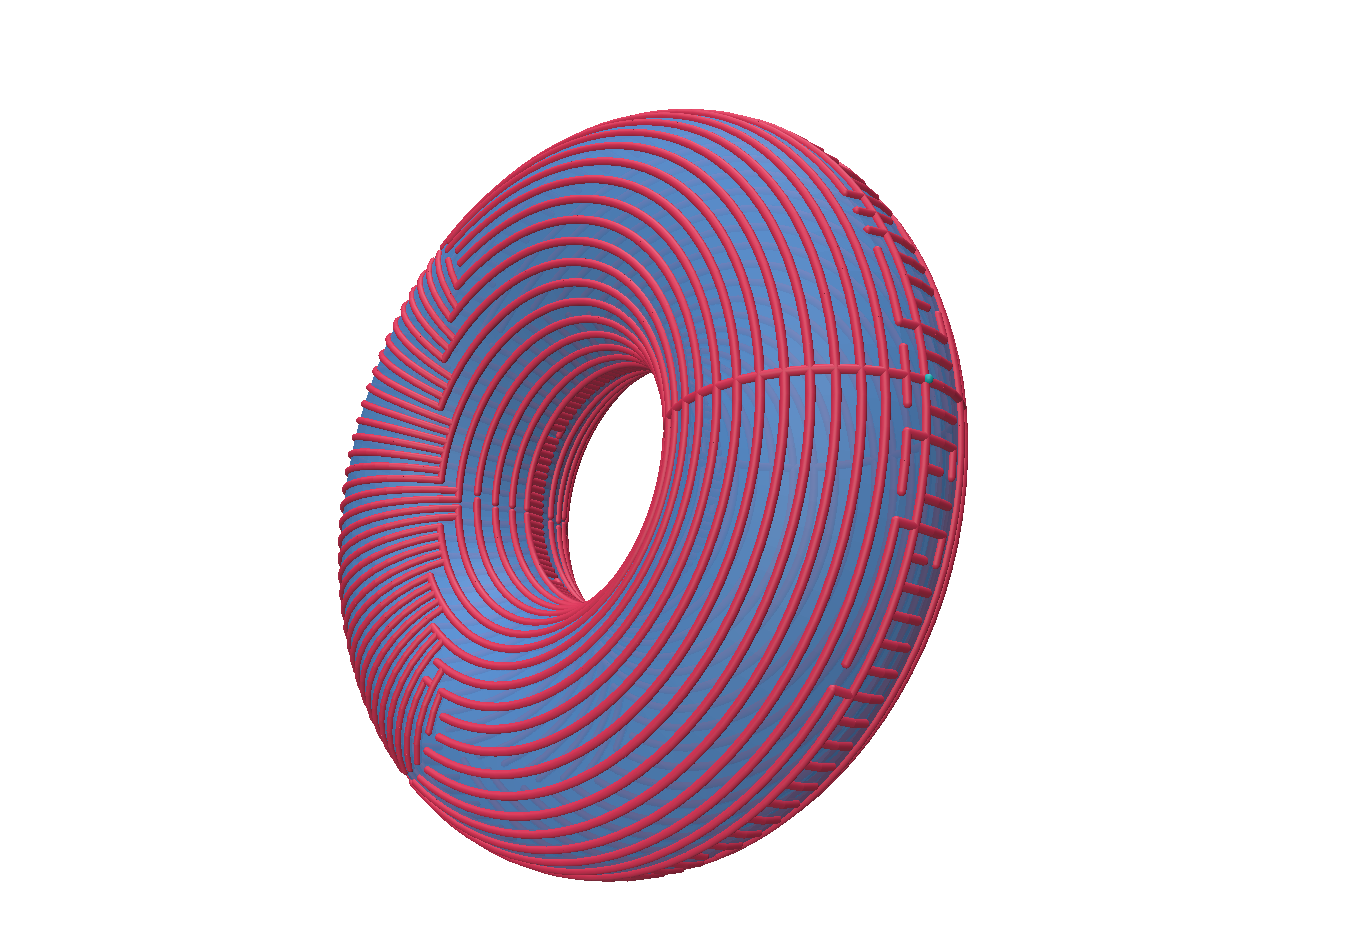
\includegraphics[width=0.4\textwidth]{arbre_couvrant_tore.PNG}
        \label{fig:subfig1}
    }
    \quad
    \subfigure[Etape 2 : $(G\setminus T)^*$ en blanc]{
        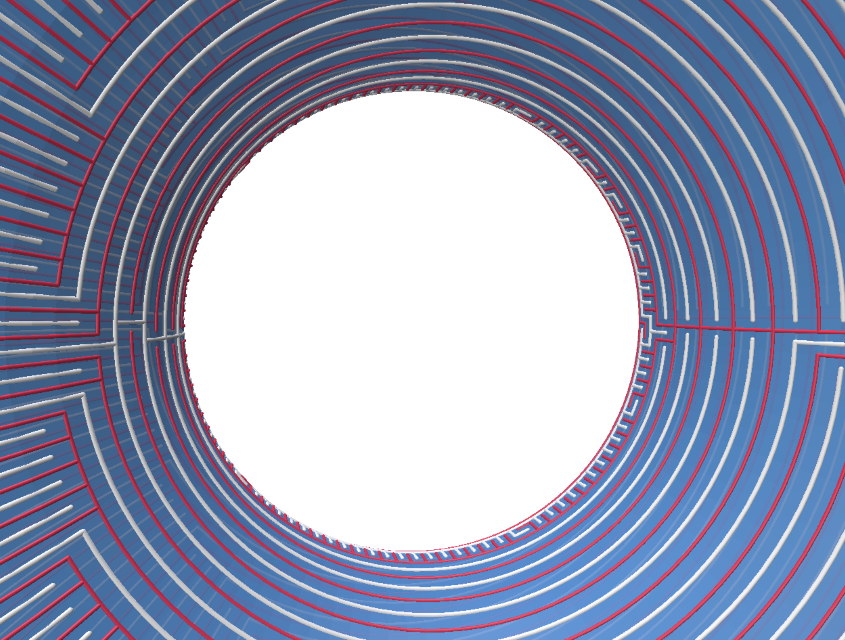
\includegraphics[width=0.4\textwidth]{show_finding_loops_eppstein2.PNG}
        \label{fig:subfig2}
    }
    
    \subfigure[Etape 3 : $T^*$ en vert et les arêtes $e^*$ utilisées dans la construction de $B$ entourées]{
        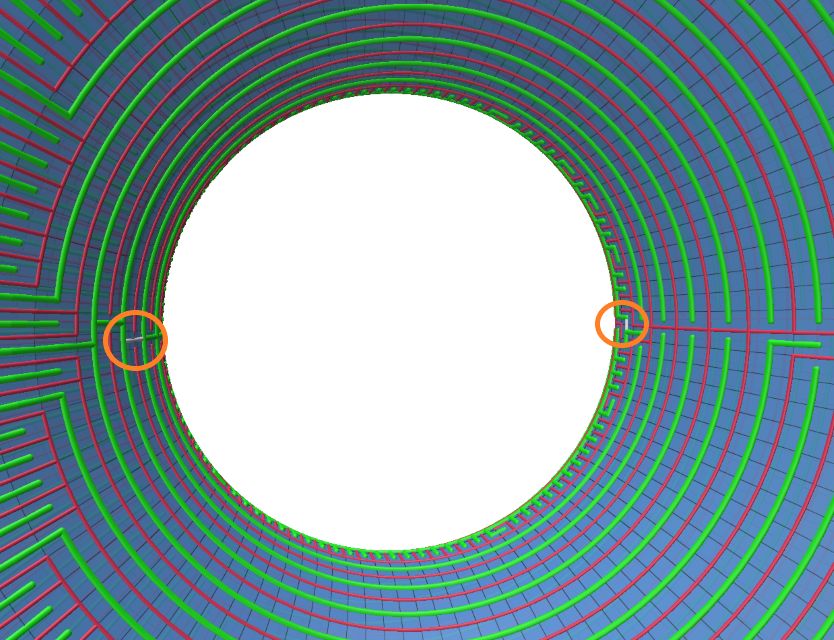
\includegraphics[width=0.4\textwidth]{show_finding_loops_eppstein4.PNG}
        \label{fig:subfig3}
    }
    \quad
    \subfigure[Etape 4 : Base homotopique $B$ la plus courte avec le point rouge pour source]{
        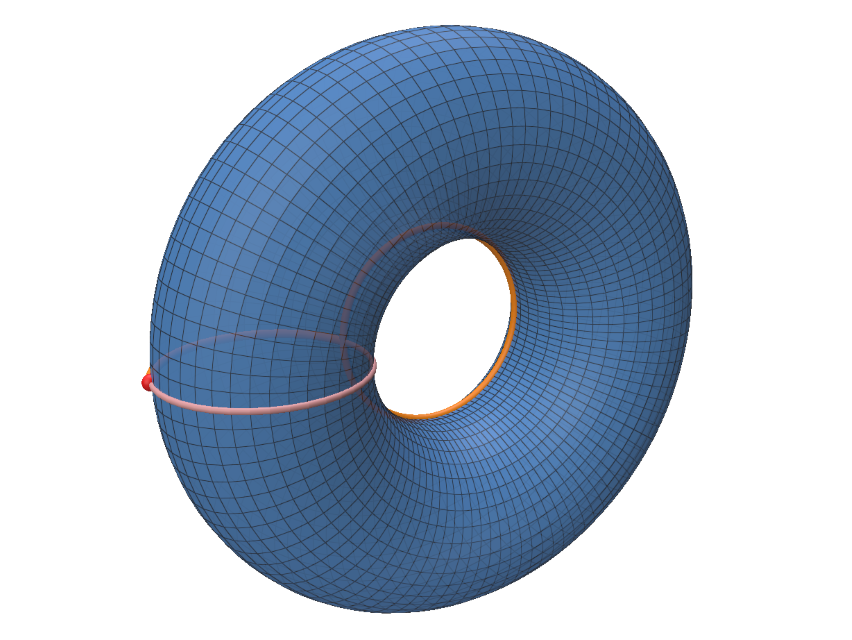
\includegraphics[width=0.4\textwidth]{shortest_loops_tore.PNG}
        \label{fig:subfig4}
    }
    \caption{Méthode pour trouver la base homotopique gloutonne avec Eppstein tree-cotree decomposition}
    \label{fig:shortest_loops_tore}
\end{figure}

\begin{figure}[!htbp]
    \centering
    \subfigure[Base homotopique sur le 2-tore]{
        \label{fig:shortest_loops_2tore}
        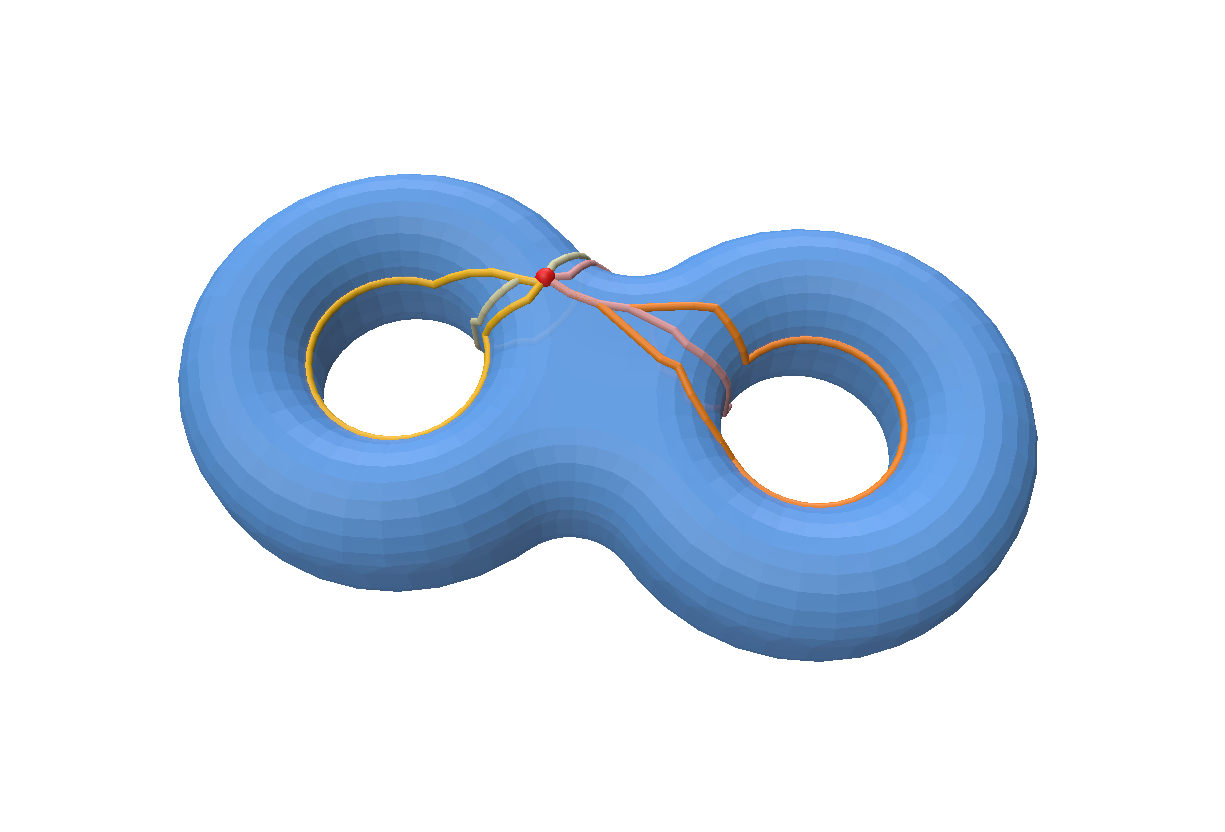
\includegraphics[width=0.4\textwidth]{shortest_loops_2tore.PNG}
    }
    \quad
    \subfigure[Base homotopique sur un cube percé]{
        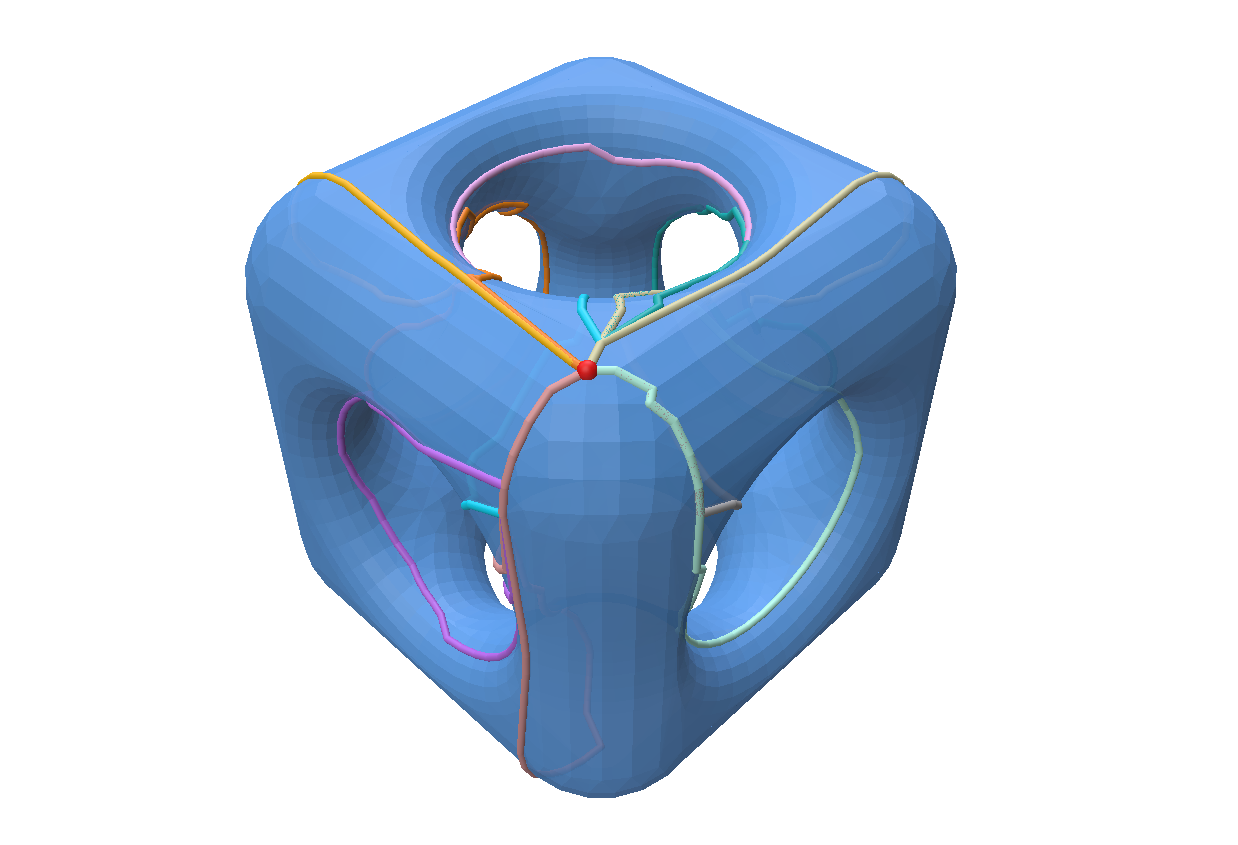
\includegraphics[width=0.4\textwidth]{loops_cubeperce.PNG}
        \label{fig:shortest_loops_cubeperce}
    }
    \caption{Bases homotopiques sur d'autres exemples}
    \label{fig:shortest_loops_others}
\end{figure}

\end{document}

% lualatex main.tex
% biber main.bcf
% lualatex main.tex